% Template for PLoS
% Version 3.1 February 2015
%
% To compile to pdf, run:
% latex plos.template
% bibtex plos.template
% latex plos.template
% latex plos.template
% dvipdf plos.template
%
% % % % % % % % % % % % % % % % % % % % % %
%
% -- IMPORTANT NOTE
%
% This template contains comments intended 
% to minimize problems and delays during our production 
% process. Please follow the template instructions
% whenever possible.
%
% % % % % % % % % % % % % % % % % % % % % % % 
%
% Once your paper is accepted for publication, 
% PLEASE REMOVE ALL TRACKED CHANGES in this file and leave only
% the final text of your manuscript.
%
% There are no restrictions o	n package use within the LaTeX files except that 
% no packages listed in the template may be deleted.
%
% Please do not include colors or graphics in the text.
%
% Please do not create a heading level below \subsection. For 3rd level headings, use \paragraph{}.
%
% % % % % % % % % % % % % % % % % % % % % % %
%
% -- FIGURES AND TABLES
%
% Please include tables/figure captions directly after the paragraph where they are first cited in the text.
%
% DO NOT INCLUDE GRAPHICS IN YOUR MANUSCRIPT
% - Figures should be uploaded separately from your manuscript file. 
% - Figures generated using LaTeX should be extracted and removed from the PDF before submission. 
% - Figures containing multiple panels/subfigures must be combined into one image file before submission.
% For figure citations, please use "Fig." instead of "Figure".
% See http://www.plosone.org/static/figureGuidelines for PLOS figure guidelines.
%
% Tables should be cell-based and may not contain:
% - tabs/spacing/line breaks within cells to alter layout or alignment
% - vertically-merged cells (no tabular environments within tabular environments, do not use \multirow)
% - colors, shading, or graphic objects
% See http://www.plosone.org/static/figureGuidelines#tables for table guidelines.
%
% For tables that exceed the width of the text column, use the adjustwidth environment as illustrated in the example table in text below.
%
% % % % % % % % % % % % % % % % % % % % % % % %
%
% -- EQUATIONS, MATH SYMBOLS, SUBSCRIPTS, AND SUPERSCRIPTS
%
% IMPORTANT
% Below are a few tips to help format your equations and other special characters according to our specifications. For more tips to help reduce the possibility of formatting errors during conversion, please see our LaTeX guidelines at http://www.plosone.org/static/latexGuidelines
%
% Please be sure to include all portions of an equation in the math environment.
%
% Do not include text that is not math in the math environment. For example, CO2 will be CO\textsubscript{2}.
%
% Please add line breaks to long display equations when possible in order to fit size of the column. 
%
% For inline equations, please do not include punctuation (commas, etc) within the math environment unless this is part of the equation.
%
% % % % % % % % % % % % % % % % % % % % % % % % 
%
% Please contact latex@plos.org with any questions.
%
% % % % % % % % % % % % % % % % % % % % % % % %

\documentclass[10pt,letterpaper]{article}
\usepackage[top=0.85in,left=2.75in,footskip=0.75in]{geometry}

% Use adjustwidth environment to exceed column width (see example table in text)
\usepackage{changepage}

% Use Unicode characters when possible
\usepackage[utf8]{inputenc}

% textcomp package and marvosym package for additional characters
\usepackage{textcomp,marvosym}

% fixltx2e package for \textsubscript
\usepackage{fixltx2e}

% amsmath and amssymb packages, useful for mathematical formulas and symbols
\usepackage{amsmath,amssymb}

% cite package, to clean up citations in the main text. Do not remove.
\usepackage{cite}

% Use nameref to cite supporting information files (see Supporting Information section for more info)
\usepackage{nameref,hyperref}

\usepackage{float}

% line numbers
\usepackage[right]{lineno}

% ligatures disabled
\usepackage{microtype}
\DisableLigatures[f]{encoding = *, family = * }

% rotating package for sideways tables
\usepackage{rotating}

% Remove comment for double spacing
%\usepackage{setspace} 
%\doublespacing

% Text layout
\raggedright
\setlength{\parindent}{0.5cm}
\textwidth 5.25in 
\textheight 8.75in

% Bold the 'Figure #' in the caption and separate it from the title/caption with a period
% Captions will be left justified
\usepackage[aboveskip=1pt,labelfont=bf,labelsep=period,justification=raggedright,singlelinecheck=off]{caption}

% Use the PLoS provided BiBTeX style
\bibliographystyle{plos2015}

% Remove brackets from numbering in List of References
\makeatletter
\renewcommand{\@biblabel}[1]{\quad#1.}
\makeatother

% Leave date blank
\date{}

% Header and Footer with logo
\usepackage{lastpage,fancyhdr,graphicx}
\usepackage{epstopdf}
\pagestyle{myheadings}
\pagestyle{fancy}
\fancyhf{}
\lhead{Royal Institute of Technology \\ DD2404 - Applied Bioinformatics}
\rhead{Bonny Wong \\ bonnyw@kthse}
\rfoot{\thepage/\pageref{LastPage}}
\renewcommand{\footrule}{\hrule height 2pt \vspace{2mm}}
\fancyheadoffset[L]{2.25in}
\fancyfootoffset[L]{2.25in}
\lfoot{\sf PLOS}

%% Include all macros below

\newcommand{\lorem}{{\bf LOREM}}
\newcommand{\ipsum}{{\bf IPSUM}}

%% END MACROS SECTION


\begin{document}
\vspace*{0.35in}

% Title must be 250 characters or less.
% Please capitalize all terms in the title except conjunctions, prepositions, and articles.
\begin{flushleft}
{\Large
\textbf\newline{DD2404 Applied Bioinformatics \\ - Signal peptide prediction}
}
\newline
% Insert author names, affiliations and corresponding author email (do not include titles, positions, or degrees).
\\
Bonny Wong
\\
\bigskip
Computer Science, Royal Institute of Technology, Stockholm, Sweden
\\
\bigskip

% Insert additional author notes using the symbols described below. Insert symbol callouts after author names as necessary.
% 
% Remove or comment out the author notes below if they aren't used.
%
% Primary Equal Contribution Note
%\Yinyang These authors contributed equally to this work.

% Additional Equal Contribution Note
% Also use this double-dagger symbol for special authorship notes, such as senior authorship.
%\ddag These authors also contributed equally to this work.

% Current address notes
%\textcurrency a Insert current address of first author with an address update
% \textcurrency b Insert current address of second author with an address update
% \textcurrency c Insert current address of third author with an address update

% Deceased author note
%\dag Deceased

% Group/Consortium Author Note
%\textpilcrow Membership list can be found in the Acknowledgments section.

% Use the asterisk to denote corresponding authorship and provide email address in note below.
%* CorrespondingAuthor@institute.edu

\end{flushleft}
% Please keep the abstract below 300 words
\section*{Abstract}
A signal peptide is a short chain of amino acids located at the start of a protein. The signal peptide is responsible for guiding the protein to its correct location. And thus knowing the existence of a signal peptide in a protein is vital information for biologists. Whether a protein contains a signal peptide can be determined experimentally. Another approach is to use machine learning to computationally predict the existence and location of these peptides. In this project two machine learning algorithms provided by the scikit-learn package for Python were trained on provided training data and used to classify previously unseen protein sequences. The results shows that the classifier can successfully predict the existence of of signal peptide with a varying rate of success ranging from 50\% up to 80\%. 

\section*{Introduction}
Proteins are large and complex molecules found throughout our body. They are responsible for a variety of vital tasks, such as carrying out chemical reactions and acting as messengers[1]. Proteins are comprised of amino acids, which forms long chains with each other. 

Many of these proteins are assembled in areas where they do not actually act in, and therefore need to be moved toward the correct areas. Signal peptides are short chains of amino acid that exists to guide these proteins on the correct path[5]. They are relevant when the location of a protein needs to be found and as such, it is important to know where these peptides are located and if they exists at all on a protein. Finding these signal peptides and be done experimentally, but there has been an increasing interest in finding them computationally instead[3]. 

Machine learning is a computer science field that essentially encompasses algorithms and methods that can learn and improve on their own. Often these algorithms learn from a set of data with known results. Once taught, the algorithm is capable of making conclusion on previously unseen data. In many cases these algorithms are taught to classify data. In a classification problem we want to determine which classes given data belong to. Often the algorithm has been trained on data with the classes already known, such algorithms are called supervised algorithms. 

In this project two supervised classification algorithms provided by scikit-learn will be used to classify proteins into two classes, proteins with signal peptide and proteins without. This paper will go through the materials used and go over the process that took place when creating the classification. 


% You may title this section "Methods" or "Models". 
% "Models" is not a valid title for PLoS ONE authors. However, PLoS ONE
% authors may use "Analysis" 
\section*{Materials and Methods}
Below follows a brief write-up of the most important tools used for this project and also the data that was used.  

\subsection*{Materials}
\paragraph{scikit-learn}
Scikit-learn is a collection of tools used for data mining and data analysis. It contains a variety of algorithms that allows data to be classified, clustering and much more. For this project tools used were its classification algorithms, the support Vector Machine (SVM) and the Naive Bayes classifier. These are supervised machine learning algorithms, which needs to be trained on data with known classes before any prediction can be made.  
\paragraph{BioPython}
BioPython is a package that eases the handling of biological data. In this project the SeqIO module was used to parse FASTA files. SeqIO parses large files quickly and provides access to the information in the FASTA headers and the sequences themselves. 
\paragraph{Training set}
The provided training set consisted of a number of FASTA files containing protein sequences positive and negative for signal peptides. 
\begin{center}
    \begin{tabular}{ | l | l | l | l |}
    \hline
    Set & Positive & Negative & Total \\ \hline
    Training set & 1320 & 1334 & 2654 \\ \hline
    \end{tabular}
\end{center}
\paragraph{Test set}
The requirements specified two proteoms to be used for testing. Ensembl Biomart was used to download the proteome from two species, Danio rerio (Zebrafish) and Gallus gallus (Red Junglefowl). The Biomart filters were used to obtain two FASTA files from each species, one with proteins positive for signal peptides and negative. These were then used in a trained classifier in order to gauge the accuracy of the classifier. 
\begin{center}
    \begin{tabular}{ | l | l | l | l |}
    \hline
    Species & Positive & Negative & Total \\ \hline
    Zebrafish & 960 & 6516 & 7476 \\ \hline
    Junglefowl & 483 & 2042 & 2525\\ \hline
    \end{tabular}
\end{center}
\paragraph{Other tools}
Other notable tools that were used for this project was Github, an online service for hosting Git repositories and Overleaf with a PLOS template for writing this paper. Google Docs was used to for the purpose of keeping notes according to 

\subsection*{Methods}
\paragraph{Stafford Noble's paper}
Stafford Noble's paper regarding how to organize computational biology project was used as a guide throughout this entire project. 
The project directories was structured according to the paper with clearly named directories and dated data and results directories. A notebook was kept and written in each time any work was being done on the project. Controls and error checking was set up to ensure robustness of the program.

\paragraph*{Machine learning}
The process of using machine learning to solve problems involves several steps. Primarily it is about gathering and preparing the data, choosing features that is distinguishing from the data and finding the correct algorithm and models to train[6]. The provided training data for this project had to be prepared before it could be fed into the algorithms given by sklearn-kit. Mainly, the data had to be structuring so that it could be transformed into a form recognizable by the machine learning algorithms. 

\paragraph*{Data preparation}
Most machine learning algorithms deals directly with numerical values. Therefore the sequences has to be turned into meaningful numbers or structures with numerical value. In the classification of text documents, the words are counted and a vector is formed were a document is represented by the word and the count of that word. The same method can be applied to protein sequences. Instead of counting words, each individual amino acid is counted. The assumption being made is that protein sequences with signal peptides may look a bit different than those without. And this difference is what a machine learning algorithm may pick up.

Since the signal peptide only occupies a small portion of the protein sequence, it is possible splice the sequences down into shorter sequence order to increase the accuracy. So instead of training or testing the whole sequence, only the first 30-40 amino acids are tested. The accuracy of this method will be shown in the results. 

Scikit-learn provides methods that counts the words or characters in a provided string. It assigns an numerical id to each unique character or word it finds and counts each occurrence, essentially forming a vector comprising of the character ids and their counts. Just counting the occurrences of character can be misleading, especially when the data set is large and can vary in size. Larger sequences would then overshadow smaller sequences, instead they need to be reduced down to their frequencies. Once this is achieved the vector of data can be used for training. 

\paragraph*{Algorithms}
Classification algorithms attempts to divide data into different classes based on certain distinguishing features. For this project two well known, but different algorithms were used, the Naive Bayes classifier and the Support Vector Machine. 

The Naive Bayes classifier is as simple classifier based on Bayes theorem. It assumes that all features are independent, which can sound like a very wrong thing to assume. But in fact the Naive Bayes classifier performs rather well on various classification problems. In essence it utilizes the Bayes theorem to calculate the probability for unclassified data to belong to a certain class it has been trained on.[7]

The SVM is a popular and useful machine learning algorithm that is highly adaptable. It is more complex than the Naive Bayes classifier. Imagine that the test data is plotted on a 2D-plane. What the algorithm attempt to do is to draw a straight line that separates the different classes of the data. In most cases drawing a straight line to separate the data is not possible, so the data has to be mapped into higher dimensional space using something called kernels. In a higher dimension it will now be possible to separate the data using a hyperplane. The hyperplane when projected back onto the 2D-plane will now appear as a line that correctly separates the data[6]. 

Given these algorithms the prepared training data was supplied to them, including a target vector consisting of the classes that each sequence belonged to. Once trained the classifiers were ready to be used for prediction. 

\paragraph*{Controls}
Some controls were established in order to assure that the results were not caused by mere noise. A method was written which simply generates completely random sequences. These random sequences were used as both training data and testing data. Error checks and messages were implemented to ensure that the program runs as stable as possible. 

% Results and Discussion can be combined.
\section*{Results}
Experiments were conducted on two classification algorithms, the Naive Bayes classifier and the SVM. Training data and test data of different lengths were used to see if it would affect the results. Below follows graphs showing the accuracy of the classifiers which were trained on all amino acids in a sequence, the first 150, 100 and 50 amino acids. The test data was split up in the same way, classifying the whole sequence, the first 30, 35, 40 and 45 amino acids. 

\paragraph*{Full training set} These results are from classifiers trained on the entire sequences in the training set. 
\begin{figure}[H] 
  \label{fig7} 
  \begin{minipage}[b]{0.6\linewidth}
    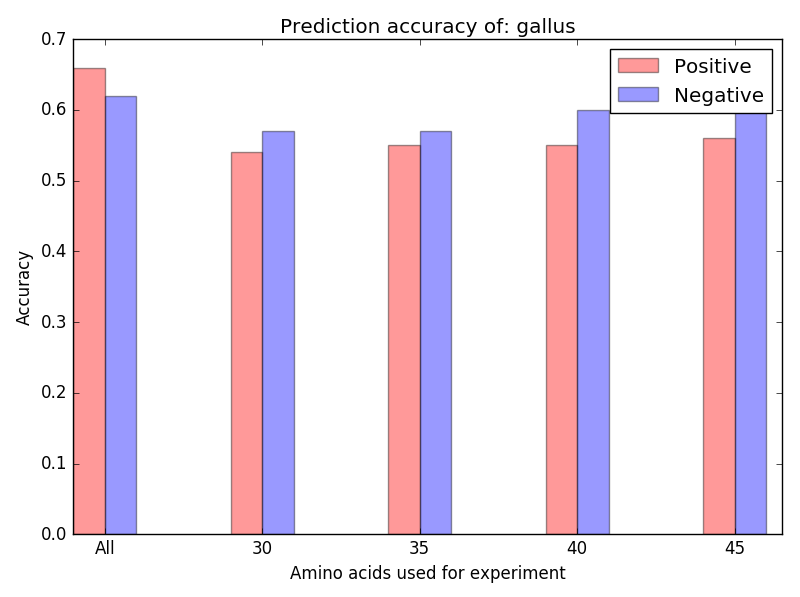
\includegraphics[width=.8\linewidth]{full_gallus_bayes} 
    \caption{Redfowl Bayes} 
    \vspace{4ex}
  \end{minipage}%%
  \begin{minipage}[b]{0.6\linewidth}
    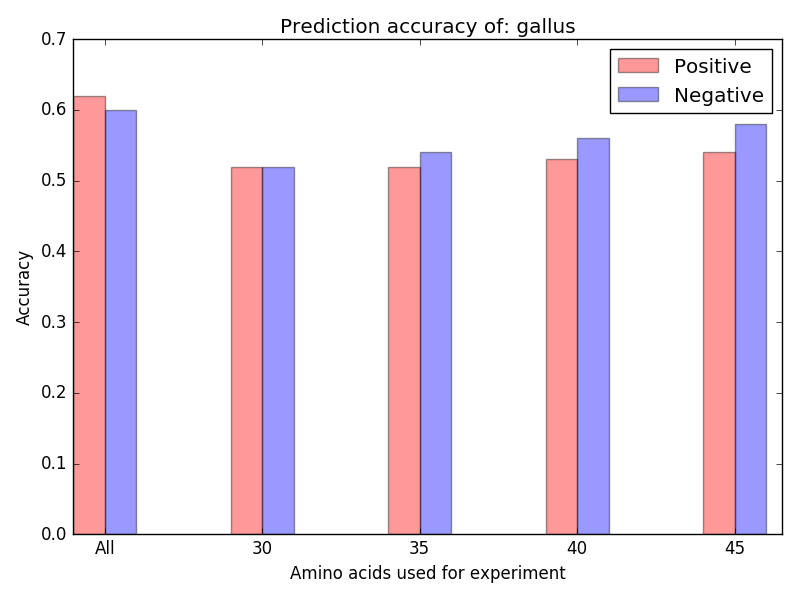
\includegraphics[width=.8\linewidth]{full_gallus_svm} 
    \caption{Redfowl SVM} 
    \vspace{4ex}
  \end{minipage} 
  \begin{minipage}[b]{0.6\linewidth}
    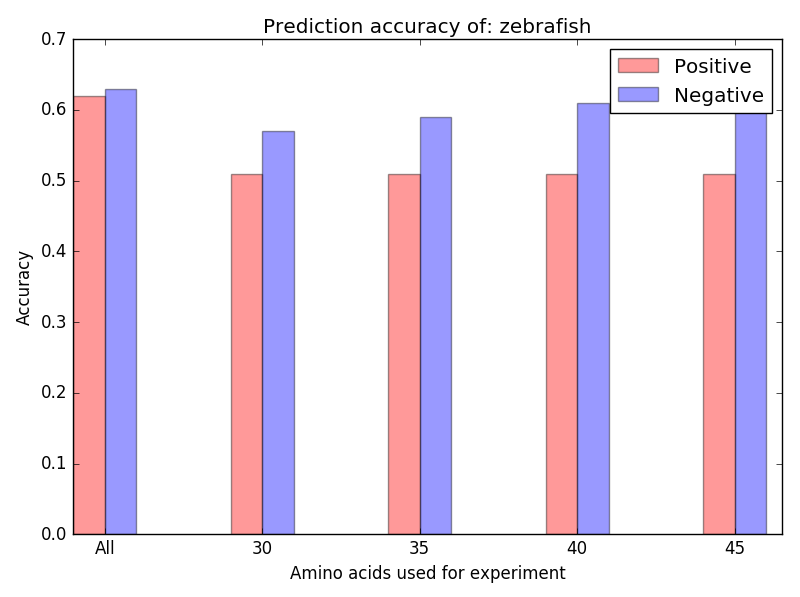
\includegraphics[width=.8\linewidth]{full_zebrafish_bayes} 
    \caption{Zebrafish Bayes} 
    \vspace{4ex}
  \end{minipage}%% 
  \begin{minipage}[b]{0.6\linewidth}
    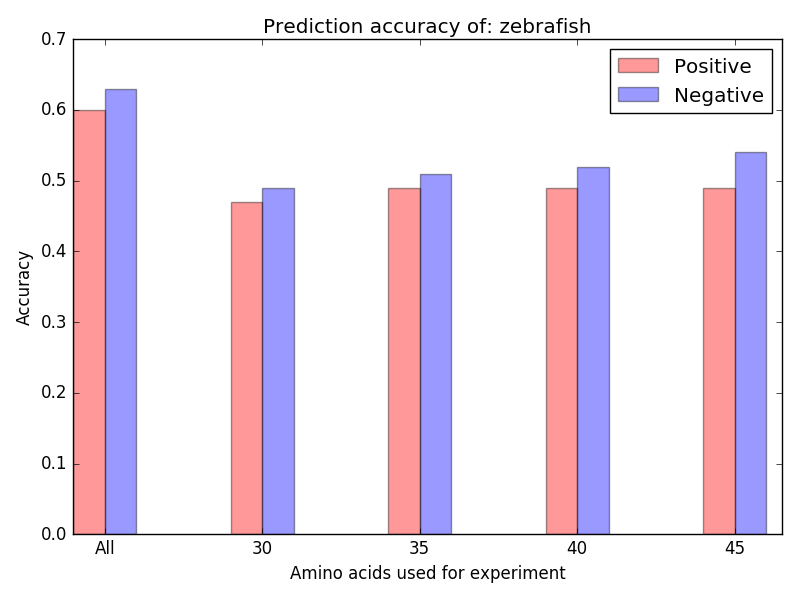
\includegraphics[width=.8\linewidth]{full_zebrafish_svm} 
    \caption{Zebrafish SVM} 
    \vspace{4ex}
  \end{minipage} 
\end{figure}

\newpage

\paragraph*{Sliced training set 150} These results are from classifiers trained on the first 150 amino acids of each sequences in the training set. 
\begin{figure}[H] 
  \label{fig7} 
  \begin{minipage}[b]{0.6\linewidth}
    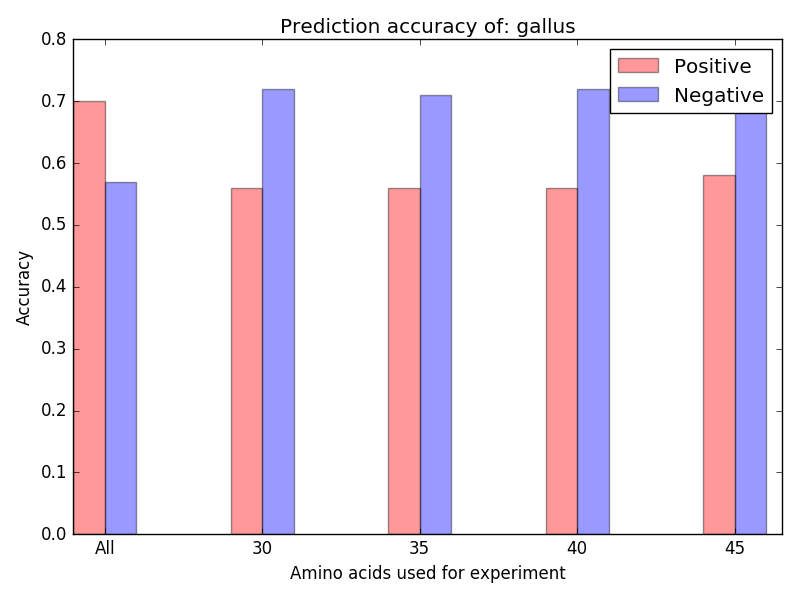
\includegraphics[width=.8\linewidth]{150_gallus_bayes} 
    \caption{Redfowl Bayes} 
    \vspace{4ex}
  \end{minipage}%%
  \begin{minipage}[b]{0.6\linewidth}
    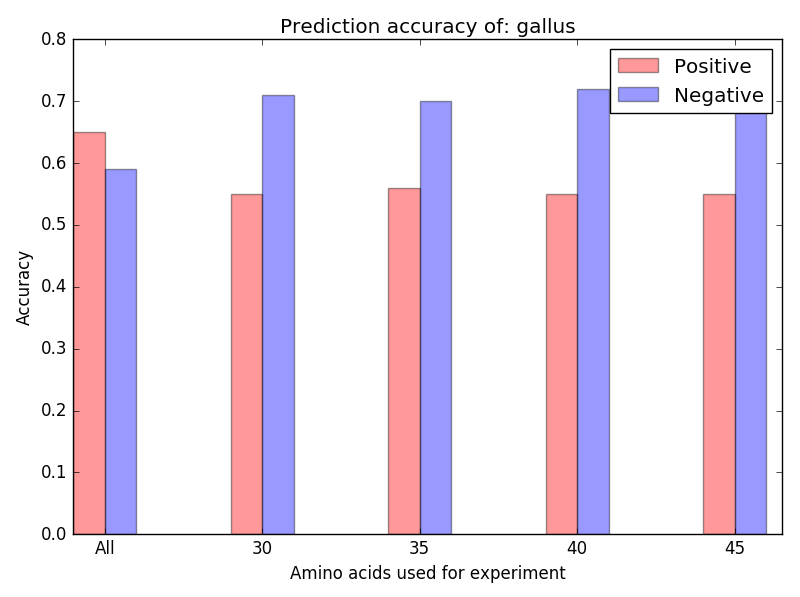
\includegraphics[width=.8\linewidth]{150_gallus_svm} 
    \caption{Redfowl SVM} 
    \vspace{4ex}
  \end{minipage} 
  \begin{minipage}[b]{0.6\linewidth}
    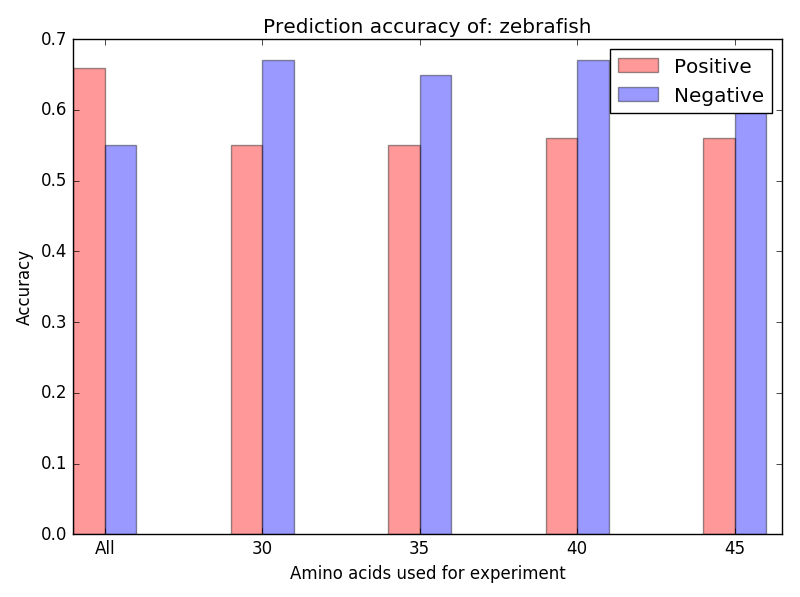
\includegraphics[width=.8\linewidth]{150_zebrafish_bayes} 
    \caption{Zebrafish Bayes} 
    \vspace{4ex}
  \end{minipage}%% 
  \begin{minipage}[b]{0.6\linewidth}
    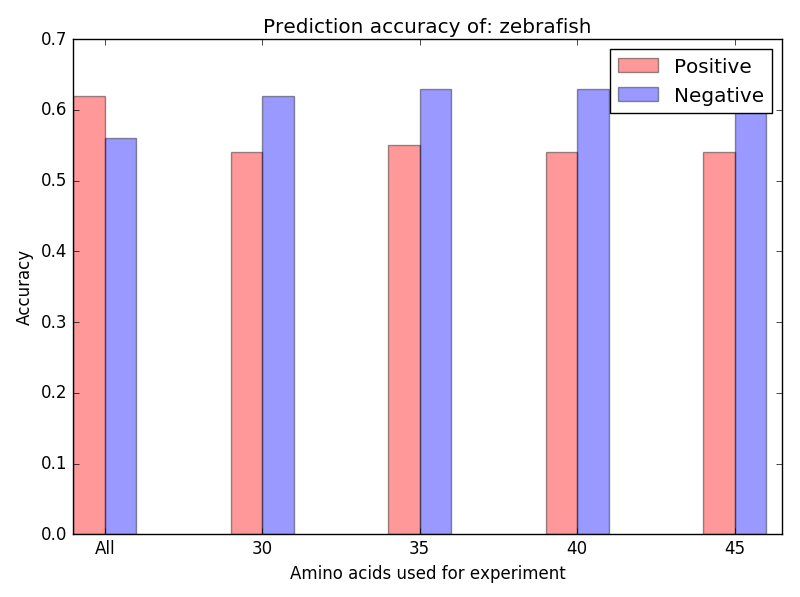
\includegraphics[width=.8\linewidth]{150_zebrafish_svm} 
    \caption{Zebrafish SVM} 
    \vspace{4ex}
  \end{minipage} 
\end{figure}

\newpage

\paragraph*{Sliced training set: 100 residues} These results are from classifiers trained on the  first 100 amino acids of each sequences in the training set. 
\begin{figure}[H] 
  \label{fig7} 
  \begin{minipage}[b]{0.6\linewidth}
    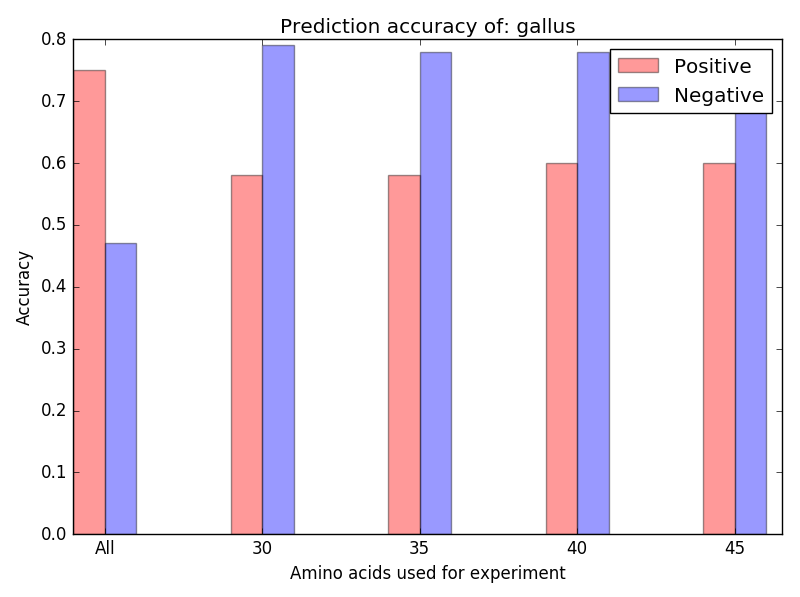
\includegraphics[width=.8\linewidth]{100_gallus_bayes} 
    \caption{Redfowl Bayes} 
    \vspace{4ex}
  \end{minipage}%%
  \begin{minipage}[b]{0.6\linewidth}
    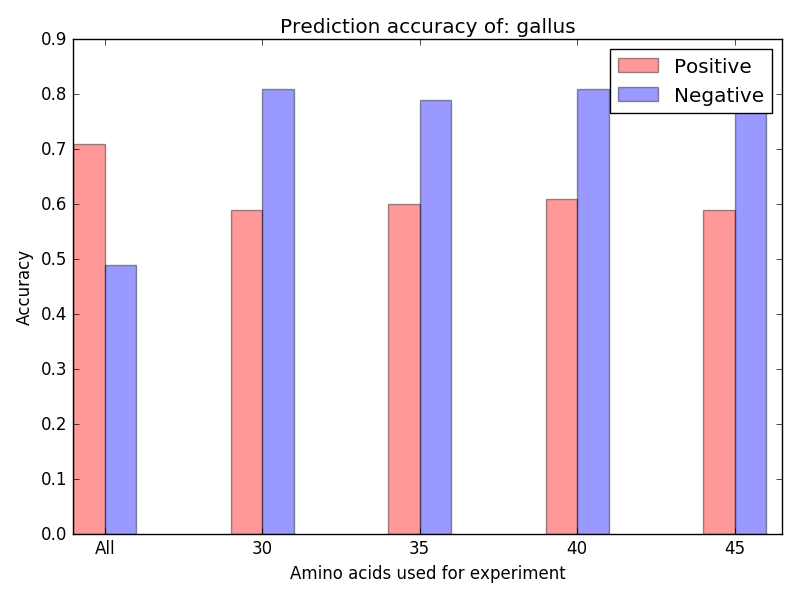
\includegraphics[width=.8\linewidth]{100_gallus_svm} 
    \caption{Redfowl SVM} 
    \vspace{4ex}
  \end{minipage} 
  \begin{minipage}[b]{0.6\linewidth}
    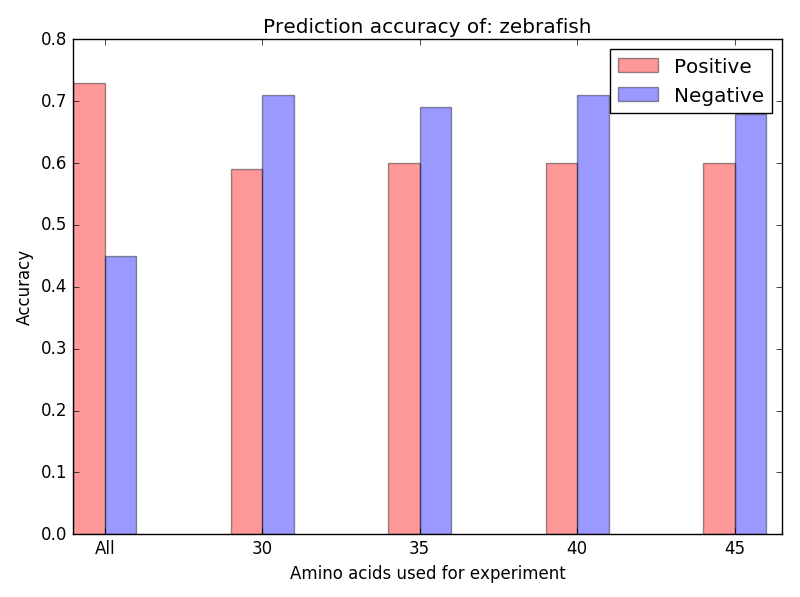
\includegraphics[width=.8\linewidth]{100_zebrafish_bayes} 
    \caption{Zebrafish Bayes} 
    \vspace{4ex}
  \end{minipage}%% 
  \begin{minipage}[b]{0.6\linewidth}
    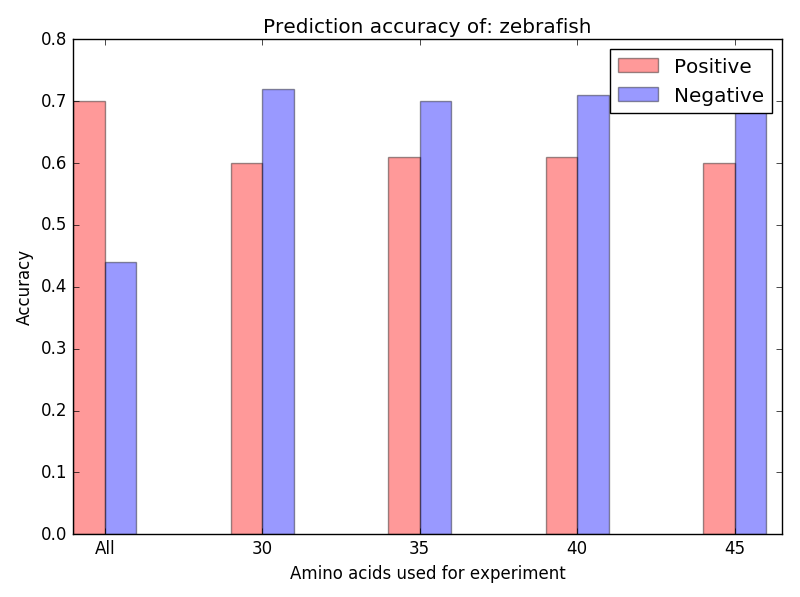
\includegraphics[width=.8\linewidth]{100_zebrafish_svm} 
    \caption{Zebrafish SVM} 
    \vspace{4ex}
  \end{minipage} 
\end{figure}

\newpage

\paragraph*{Sliced training set, 50 residues} These results are from classifiers trained on the first 50 amino acids of each sequences in the training set. 
\begin{figure}[H] 
  \label{fig7} 
  \begin{minipage}[b]{0.6\linewidth}
    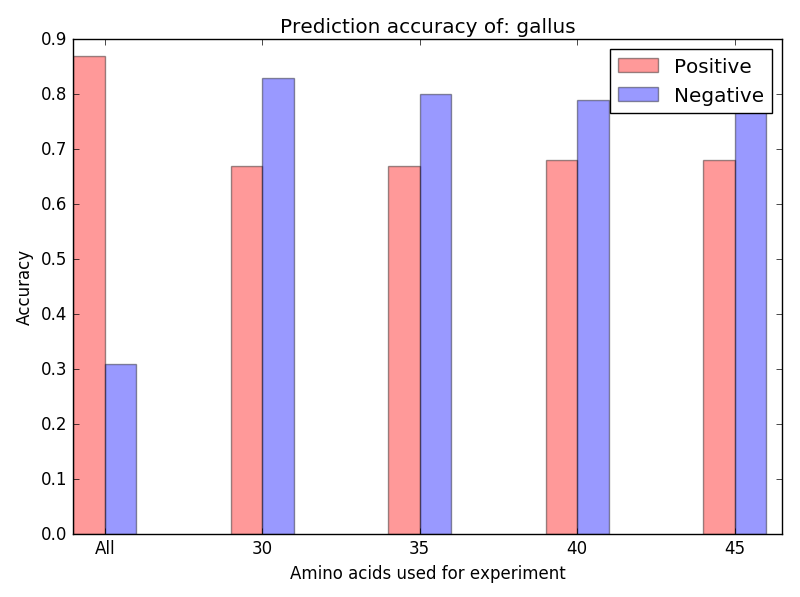
\includegraphics[width=.8\linewidth]{50_gallus_bayes} 
    \caption{Redfowl Bayes} 
    \vspace{4ex}
  \end{minipage}%%
  \begin{minipage}[b]{0.6\linewidth}
    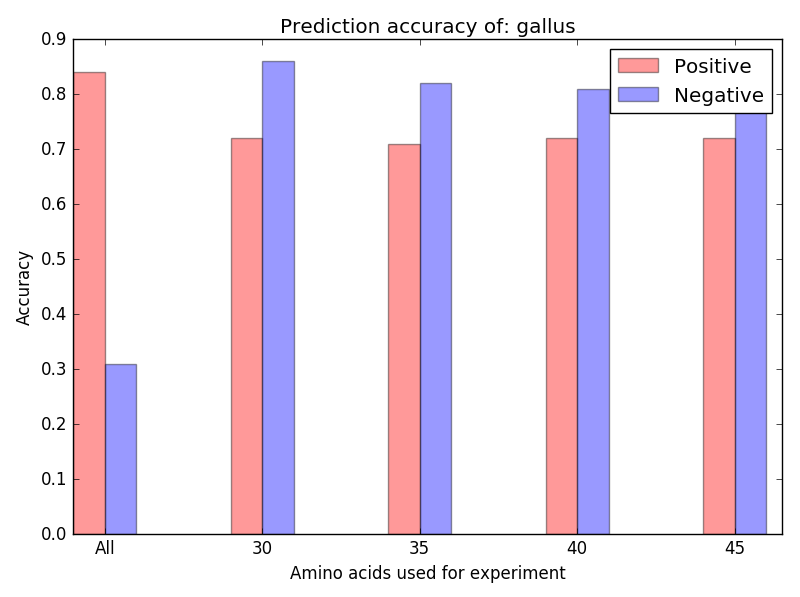
\includegraphics[width=.8\linewidth]{50_gallus_svm} 
    \caption{Redfowl SVM} 
    \vspace{4ex}
  \end{minipage} 
  \begin{minipage}[b]{0.6\linewidth}
    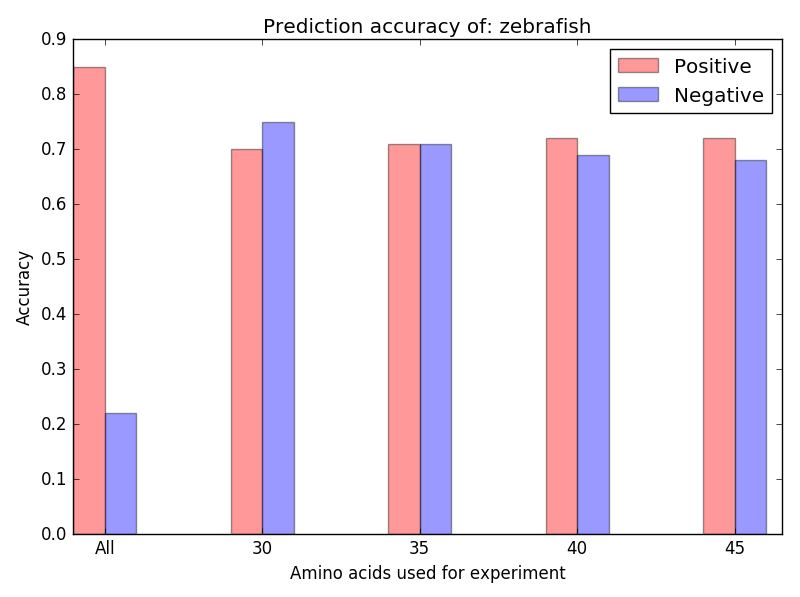
\includegraphics[width=.8\linewidth]{50_zebrafish_bayes} 
    \caption{Zebrafish Bayes} 
    \vspace{4ex}
  \end{minipage}%% 
  \begin{minipage}[b]{0.6\linewidth}
    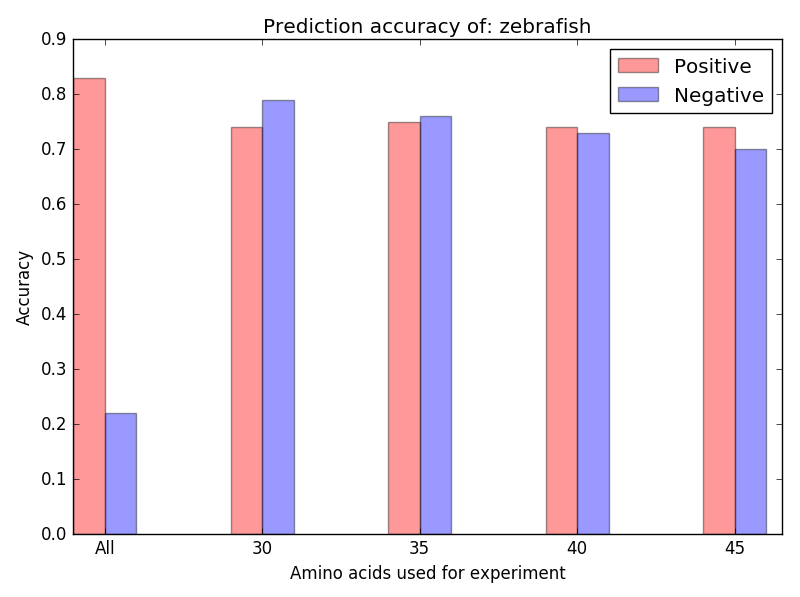
\includegraphics[width=.8\linewidth]{50_zebrafish_svm} 
    \caption{Zebrafish SVM} 
    \vspace{4ex}
  \end{minipage} 
\end{figure}


\section*{Discussion and Conclusion}
The results show an accuracy that hovers around the 50-70\% area depending on method used and the amount of residues that are accounted for, occasionally reaching 80\% accuracy. While not very good at classifying proteins, it manages to do it correctly in more than majority of the cases. The accuracy varied highly depending on the number of amino acids that are used both in the training set and the testing set. 

Since a signaling sequence is rather short, 5-30 amino acids, it made sense that the tests involving sliced training sequences and sliced test sequences had higher accuracy than tests on full sequences and full proteins. Consequently testing a full sequence against a classifier trained on only the first 50 amino acids shows very bad results as seen in figure 13, 14, 15 and 16. However the shorter test sequences fared much better, resulting over 70\% chance to correctly identify both sequences with and without a signal peptide. This trend can be seen on both the classifiers. 

In the cases where the whole training set was used the simpler Naive Bayes classifier performed slightly better on the negative test cases, managing to beat the SVM. As smaller portions of sequences in the the training set and testing set are used, the SVM starts to outperform the Bayes classifier. 


\subsection*{Improvements}
There are a large number of improvements that could be added to the project. One of the more obvious improvements is to train the classifier on more data. At this moment the classifier is retrained on the same training after each prediction. If a much larger training set is used, one could constantly train the classifier and store it in a server, allowing test to be ran against it. That of course would require fast ways to predict and retrieve the data.

The classifiers has a lot of parameters that can be changed. Sometimes the difference between a bad and a good classification is heavily dependent on what kind of parameters that are fed into the algorithms. Tweaking these parameters would be one important thing to do when attempting to increase the accuracy of the prediction. 

Using another method to find and represent the features of a protein sequence would also likely prove beneficial. The current approach simply tokenizes the sequence by counting each amino acid and finding out how often they appear in a sequence. This approach is rather naive, as it assumes there are no relation between the amino acids. Looking at groups of amino acids based on certain requirements if they exist would likely be a much better approach. The sequence logo of signal peptides also suggest there are relations between the amino acids that stands out. 

\subsection*{Conclusion}
The classifiers has managed to classify proteins with a large spread in accuracy. The rate of success is highly dependent on how many amino acids that are being used. By limiting the sequences in the training set and the test set to the same length as an average sinal peptide a high degree of accuracy was reached. However that accuracy vanished if the full sequences are used. 

This project has shown that better algorithms, or a better choice in features to train is required in order to obtain better results. 

\nolinenumbers

%\section*{References}
% Either type in your references using
% \begin{thebibliography}{}
% \bibitem{}
% Text
% \end{thebibliography}
%
% OR
%
% Compile your BiBTeX database using our plos2015.bst
% style file and paste the contents of your .bbl file
% here.
% 
\begin{thebibliography}{10}
\bibitem{bib1}
National Institute of Health - What are proteins and what do they do?
http://ghr.nlm.nih.gov/handbook/howgeneswork/protein

\bibitem{bib2}
William Stafford Noble, A Quick Guide to Organizing Computational Biology Projects
http://journals.plos.org/ploscompbiol/article?id=10.1371/journal.pcbi.1000424\#s5

\bibitem{bib3}
DD2404 Applied Bioinformatics project description
https://www.kth.se/social/course/DD2404/subgroup/ht-2015-appbio15/page/predicting-signal-peptides-2/

\bibitem{bib4}
SignalP V1.1 Signal peptide lengths
http://www.cbs.dtu.dk/services/SignalP-1.1/sp\_data.html

\bibitem{bib5}
Yale School of Medicine - Cell Biology: Secretion and Endocytosis
http://medcell.med.yale.edu/lectures/secretion\_endocytosis.php

\bibitem{bib6}
Stephen Marsland, Machine Learning: An Algorithmic Perspective

\bibitem{bib7}
Dell Software, Naive Bayes Classifier
http://documents.software.dell.com/Statistics/Textbook/Naive-Bayes-Classifier

\end{thebibliography}



\end{document}

